%%%%%%%%%%%%%%%%%%%%%%%%%%%%%%%%%%%%%%%%%
% "ModernCV" CV and Cover Letter
% LaTeX Template
% Version 1.1 (9/12/12)
%
% This template has been downloaded from:
% http://www.LaTeXTemplates.com
%
% Original author:
% Xavier Danaux (xdanaux@gmail.com)
%
% License:
% CC BY-NC-SA 3.0 (http://creativecommons.org/licenses/by-nc-sa/3.0/)
%
% Important note:
% This template requires the moderncv.cls and .sty files to be in the same 
% directory as this .tex file. These files provide the resume style and themes 
% used for structuring the document.
%
%%%%%%%%%%%%%%%%%%%%%%%%%%%%%%%%%%%%%%%%%

%----------------------------------------------------------------------------------------
%	PACKAGES AND OTHER DOCUMENT CONFIGURATIONS
%----------------------------------------------------------------------------------------

\documentclass[11pt,a4paper,sans]{moderncv} % Font sizes: 10, 11, or 12; paper sizes: a4paper, letterpaper, a5paper, legalpaper, executivepaper or landscape; font families: sans or roman

\moderncvstyle{casual} % CV theme - options include: 'casual' (default), 'classic', 'oldstyle' and 'banking'
\moderncvcolor{red} % CV color - options include: 'blue' (default), 'orange', 'green', 'red', 'purple', 'grey' and 'black'

\usepackage{contour}% http://ctan.org/pkg/contour
\contourlength{0.01em}% Smaller radius

\usepackage{lipsum} % Used for inserting dummy 'Lorem ipsum' text into the template
\usepackage[T2A]{fontenc}
\usepackage[scale=0.825]{geometry} % Reduce document margins

\usepackage{listings}
\usepackage{color}

\definecolor{dkgreen}{rgb}{0,0.6,0}
\definecolor{gray}{rgb}{0.5,0.5,0.5}
\definecolor{mauve}{rgb}{0.58,0,0.82}

\lstset{frame=tb,
	language=Java,
	aboveskip=3mm,
	belowskip=3mm,
	showstringspaces=false,
	columns=flexible,
	basicstyle={\small\ttfamily},
	numbers=none,
	numberstyle=\tiny\color{gray},
	keywordstyle=\color{blue},
	commentstyle=\color{dkgreen},
	stringstyle=\color{mauve},
	breaklines=true,
	breakatwhitespace=true,
	tabsize=3
}

\setlength{\hintscolumnwidth}{3cm} % Uncomment to change the width of the dates column
\usepackage{graphicx}
%\setlength{\makecvtitlenamewidth}{10cm} % For the 'classic' style, uncomment to adjust the width of the space allocated to your name

\graphicspath{ {screens/} }

\makeatletter
\newcommand\@pnumwidth{1.55em}
\newcommand\@tocrmarg{2.55em}
\newcommand\@dotsep{4.5}
\makeatother
\usepackage{titletoc}

\makeatletter
\setlength\columnsep{20pt}
\setcounter{tocdepth}{0}
\newcommand\contentsname{Contents}
\newcommand\tableofcontents{%
	\addtocontents{toc}{\protect\setcounter{tocdepth}{0}}
	\section*{\contentsname}
	\addtocontents{toc}{\protect\setcounter{tocdepth}{2}}
	\@starttoc{toc}%
}
\usepackage{titletoc}
\titlecontents*{section}[0pt]
{}{}{}
{\hfill \thecontentspage \newline}[\ \newline\ ][]
\renewcommand\l@subsection[2]{}
\makeatother

%----------------------------------------------------------------------------------------
%	NAME AND CONTACT INFORMATION SECTION
%----------------------------------------------------------------------------------------

\firstname{Mass Site} % Your first name
\familyname{Visitor} % Your last name

% All information in this block is optional, comment out any lines you don't need
\title{User's Guide}
\address{}{}
\mobile{}
\email{}
\homepage{}{} % The first argument is the url for the clickable link, the second argument is the url displayed in the template - this allows special characters to be displayed such as the tilde in this example
%\extrainfo{additional information}
%\photo[70pt][0.4pt]{pictures/picture} % The first bracket is the picture height, the second is the thickness of the frame around the picture (0pt for no frame)

%----------------------------------------------------------------------------------------

\begin{document}
%\pagenumbering{alph}
\fontencoding{OT1}
\makecvtitle % Print the CV title

\tableofcontents
\newpage
%----------------------------------------------------------------------------------------
%	USAGE SECTION
%----------------------------------------------------------------------------------------
\setlength{\hintscolumnwidth}{1.7cm}
\section{General usage and description}
%\pagenumbering{arabic}


\cvitem{\textit{General features}}{Mass Site Visitor (MSV) is a traffic bot, a program, designed to generate large amounts of traffic to websites of your choice through the list of proxies in a multi-threaded way. This software uses your PC to run hidden browser sessions concurrently in the background, directs their traffic to the target websites through proxies, so that each such session has a unique distinct IP address, appearing to be from anywhere in the world.\newline You can set referrers and user agents, which along with proxies will be randomly selected to create a browser session. \textbf{Referrers}, \textbf{user agents} and \textbf{proxies} should be stored in a text-file and can be appended to an already loaded list in the program by pressing the \textbf{'Load the ... list' button}. Proxy list format is discussed in the appropriate section below in this guide. \newline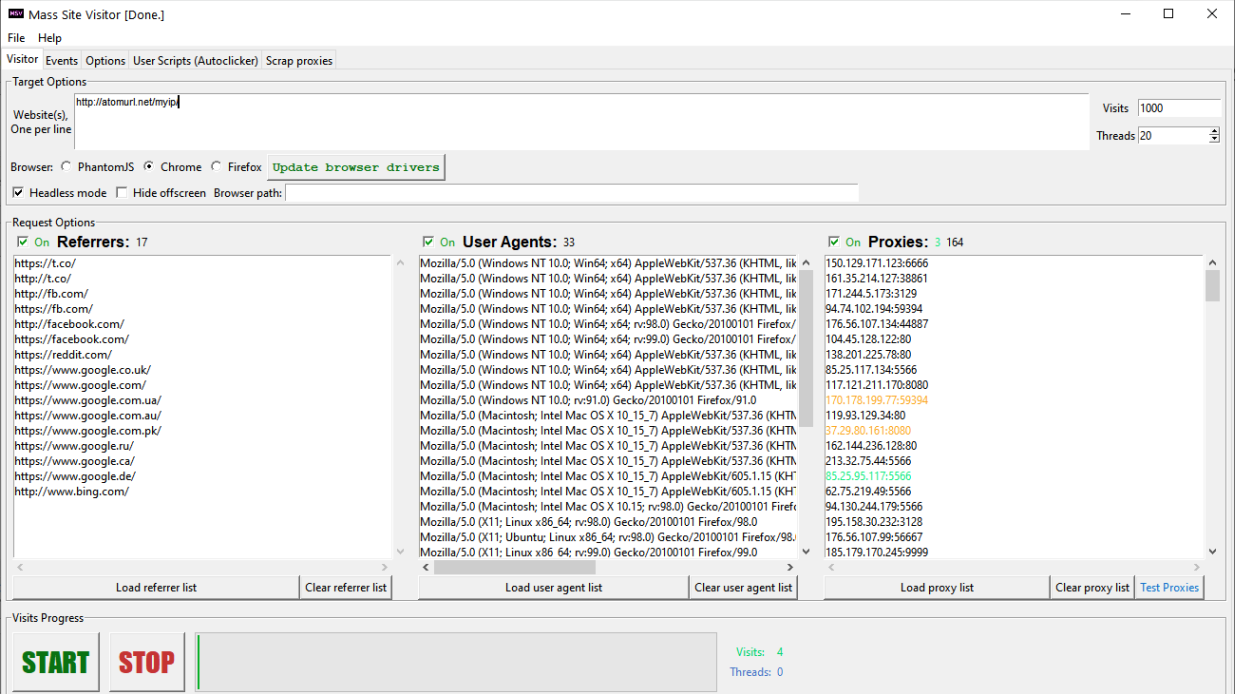
\includegraphics[scale=0.45]{screen1}}


\cvitem{\textit{Settings}}{You can save screenshots of visits, set up window sizes, browser locales, select referrer spoofing for JavaScript-based analytics, enable Alexa addon in the browser, and more by enabling corresponding settings in the Options tab\newline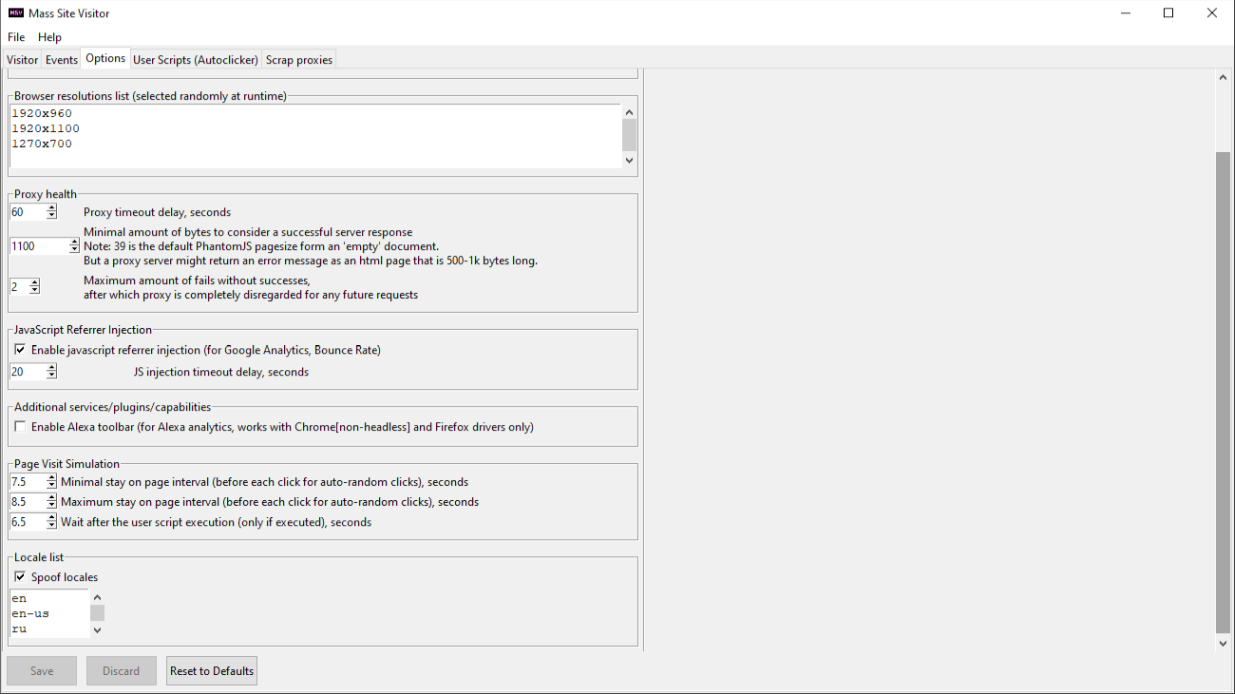
\includegraphics[scale=0.45]{screen3}}

\cvitem{\textit{Scripted behavior, autoclicks}}{You can setup user behavior simulation either by setting MSV to click on a particular link in the page, or perform random scrolling and clicking. Particular clicking (User Scripts section of the User Scripts tab) will have a priority and will be executed before the random clicking and scrolling (Auto-Random Behavior section of the User Scripts tab), if both are enabled. It will be executed once per visit, in this case, and then the auto-random logic executed the amount of times set in the options of the feature (Total clicks), with one auto-random scroll executed after each auto-random click, if enabled. After which, the particular visit will be considered complete. Wait periods between each autoclick (random or particular) are defined in the Options tab,  Page Visit Simulation section.\newline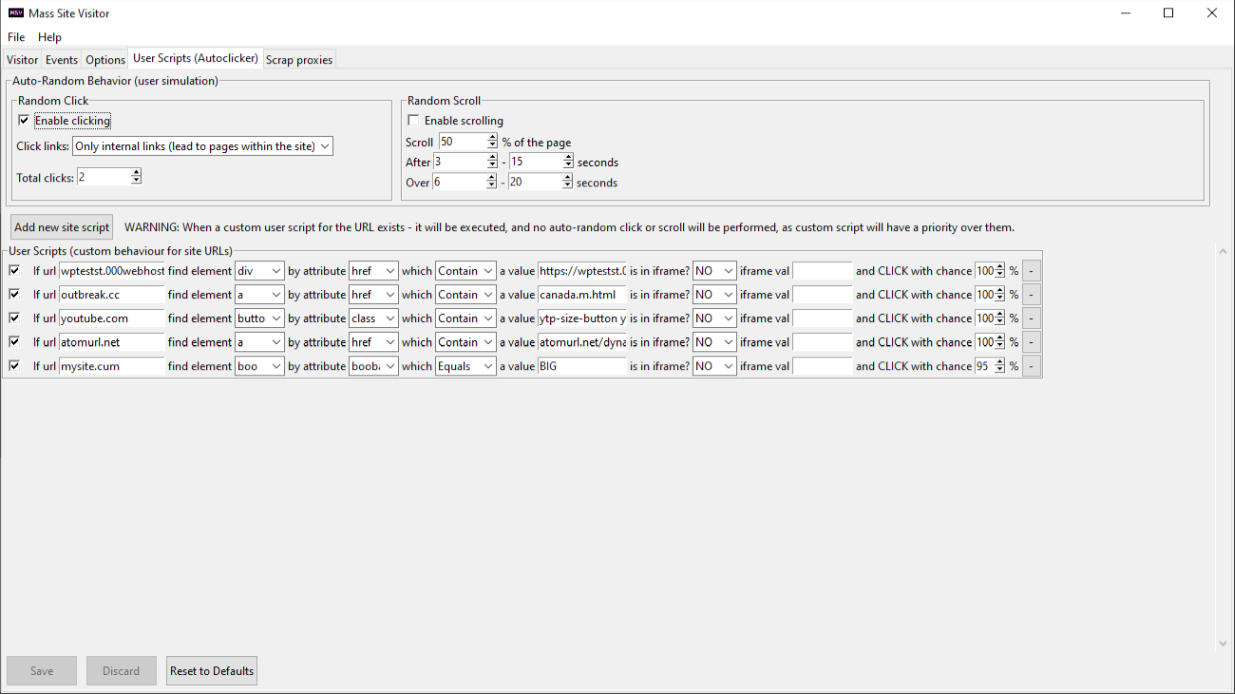
\includegraphics[scale=0.45]{screen6}}


\cvitem{\textit{Filtering out proxies, that didn't work during the last session}}{There is an ability to filter out non-responsive proxies from the ones that work, and save them to file (\textbf{Settings -  Export Healthy Proxies} after running the proxy test), use this feature often, it will help you to work with good, working proxies during the consecutive program runs.\newline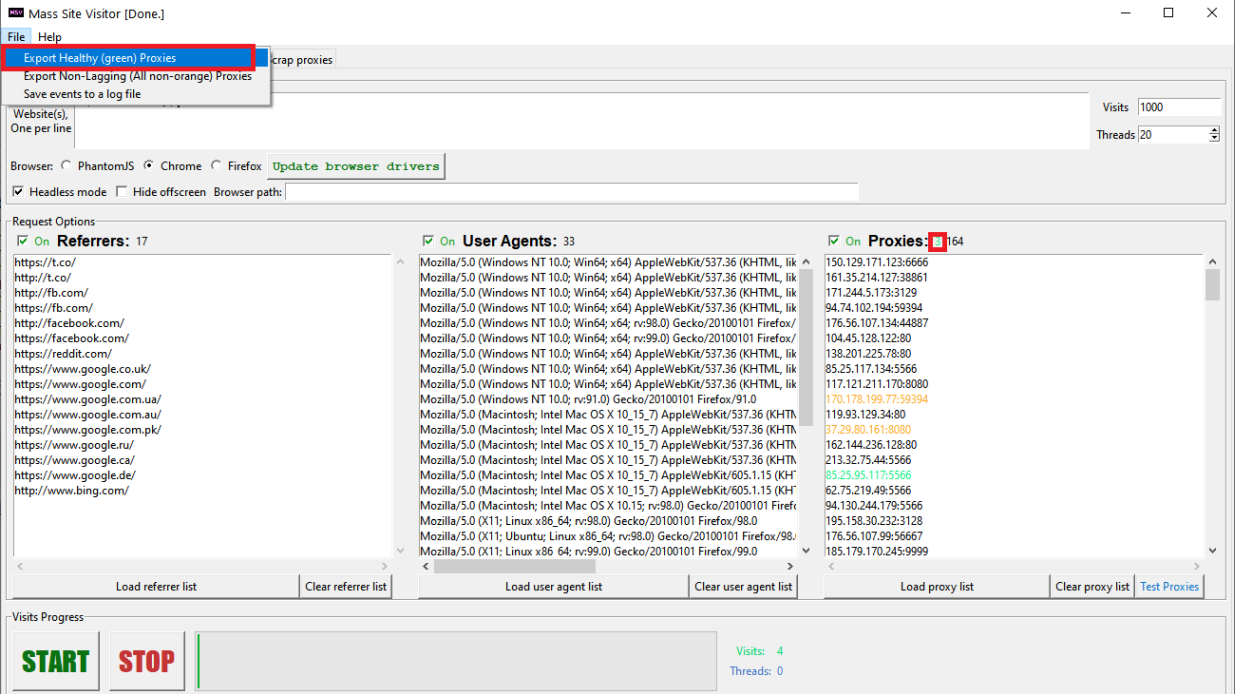
\includegraphics[scale=0.45]{screen5}}


\cvitem{\textit{Scraping public proxies}}{If you don't have a proxy list of your own, and the one supplied with MSV isn't satisfactory (with time those proxies might cease to work), there is an ability to scrap public proxies from the web,\textbf{ Settings - Import Proxies from the web}, if you are scraping proxies from the web, you don't have to worry about adding the proxy type for a socks proxy, program will save all the info in the right format.\newline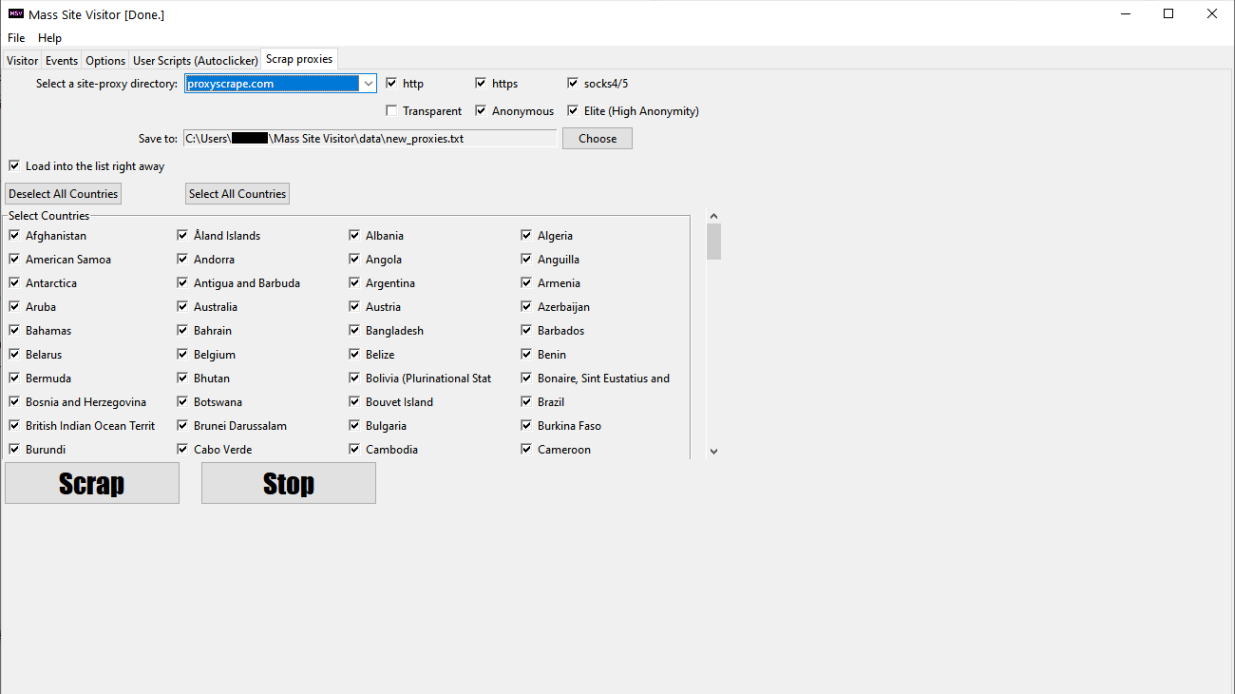
\includegraphics[scale=0.45]{screen4}}


\cvitem{\textit{Additional features, conveniences}}{The \textbf{log of events}, that happened in a context of the program is available for the user to study. It will contain messages about the proxy scraping process, as well as the process of sending traffic through proxies to the target website and bot clicks.\newline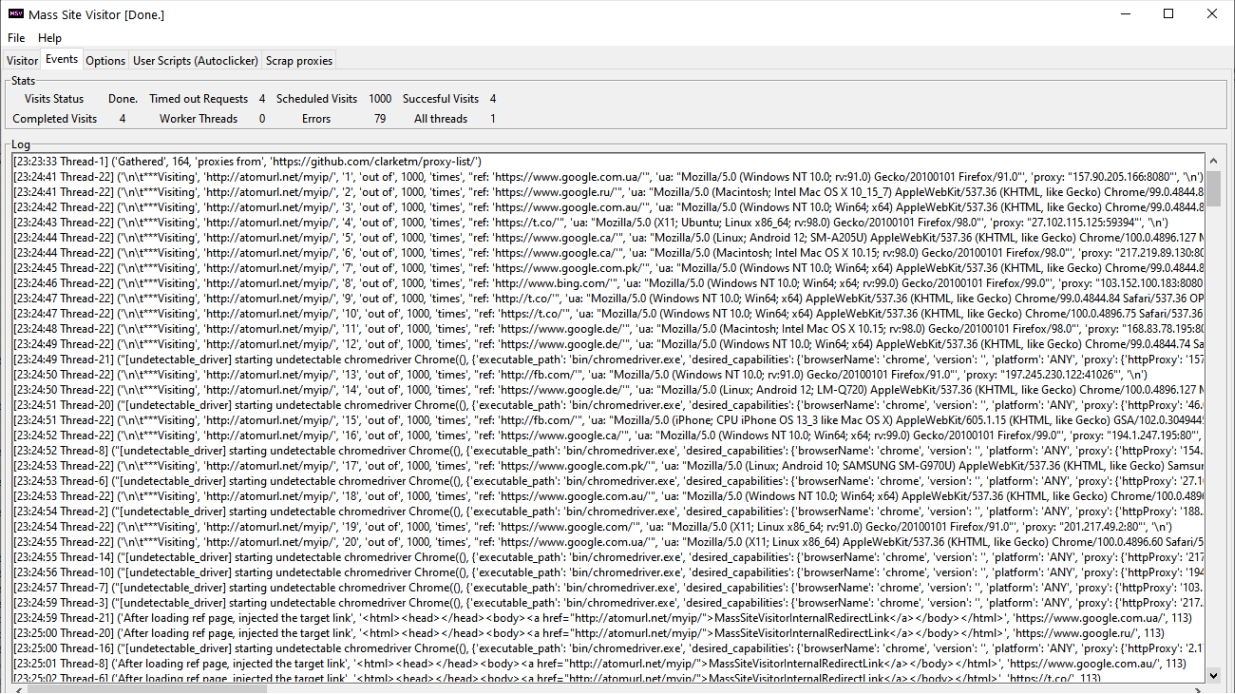
\includegraphics[scale=0.45]{screen2}}

%----------------------------------------------------------------------------------------
%	Autoclicker SECTION
%----------------------------------------------------------------------------------------

\section{Autoclicker usage and tips}
\cvitem{\textbf{General case}}{This feature relies on html elements and their attributes as defined in the web-page's html code, to find and click the link/button/banner of your choice. That's why you would have to use your browser's \textbf{Element Inspector} (or equivalent, literally every browser has such tool) to get the data you need and then paste into the MSV Options tab. In this Firefox example you can see that a context menu for any web-page element has \textit{Inspect Element} item in it:\newline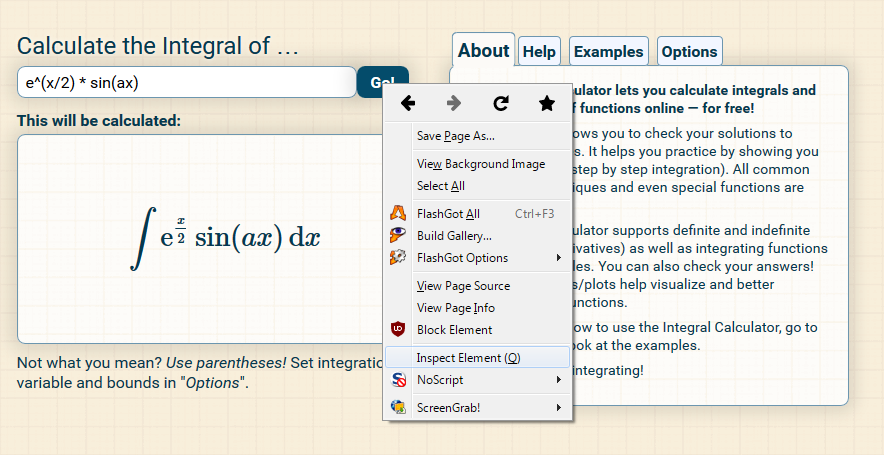
\includegraphics[scale=0.6]{instructions1}} 
\cvitem{}{After a click on this context menu item somewhere to the side or bottom of the browser's window you'll see a construct with all the html tags and their attributes, and the one you clicked to "inspect" is highlighted right away, like the following:\newline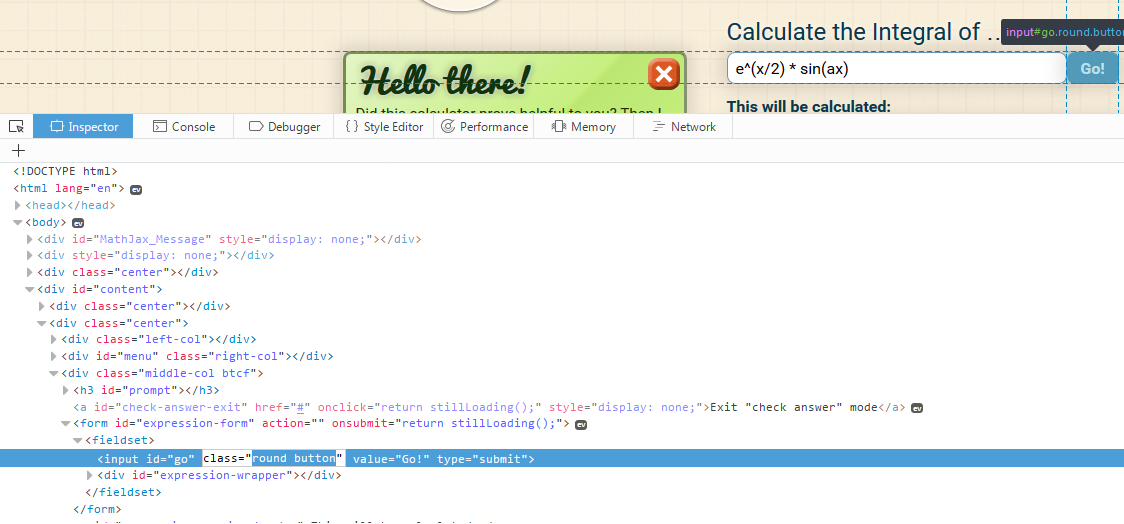
\includegraphics[scale=0.525]{instructions2}} 
\cvitem{}{Pay attention to the highlighted line in the Element Inspector and the corresponding highlighted button in the browser's page view. Element (tag) \textit{input} corresponds to that button. And to precisely identify this exact button we would use its \textit{class} attribute. Pay attention to what goes into which field in MSV options (you need to click the \textbf{Add new site script} button beforehand). Ignore the iframe-ralated options for now (we'll consider that special case later):\newline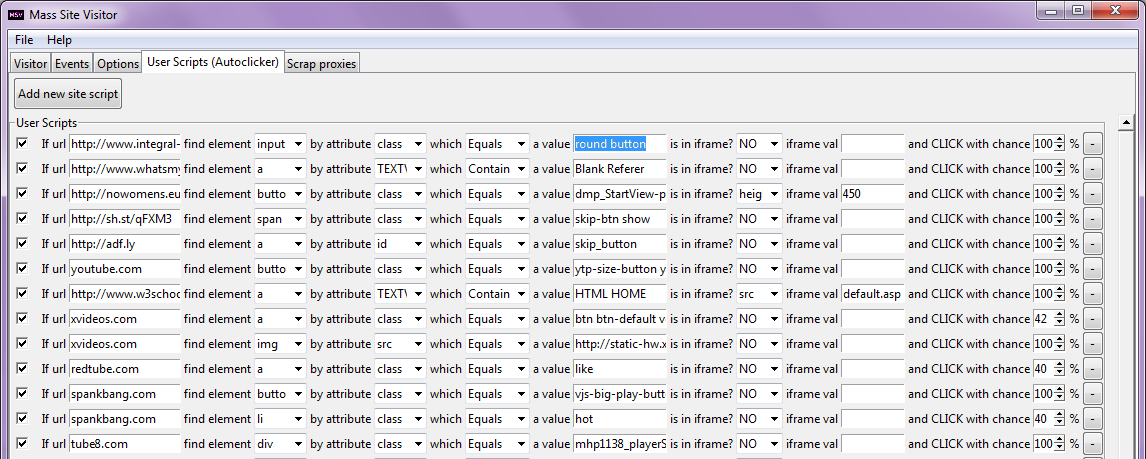
\includegraphics[scale=0.5]{instructions3}} 
\cvitem{}{There are several attributes and elements available in drop-down menus to choose from, and even if the exact kind of attribute or element you need is not present in the default choice, you can \textbf{type in the needed string yourself}, drop-down menus are typable. The special \textit{TEXTVAL} attribute is used when you want to search for a link with some inner text that looks in html like the following: <a ....>CLICK ME!</a>} 
\cvitem{}{Chance to click will be useful to you if you don't want every successful visit to click the element you're interested in (some video hosting sites allow anonymous users to leave ratings, but it would be kind of suspicious if right after video was uploaded it got as many different ratings as it got views, naturally not all the viewers bother to like/rate the video after watching it.)} 
\cvitem{\textbf{Inside iframe}}{Since iframe is used to embed some other web-page within the current page, elements inside that iframe are not considered part of the main page (the one, at which URL you are currently). That's where those last two textfields of the click script come to play.\newline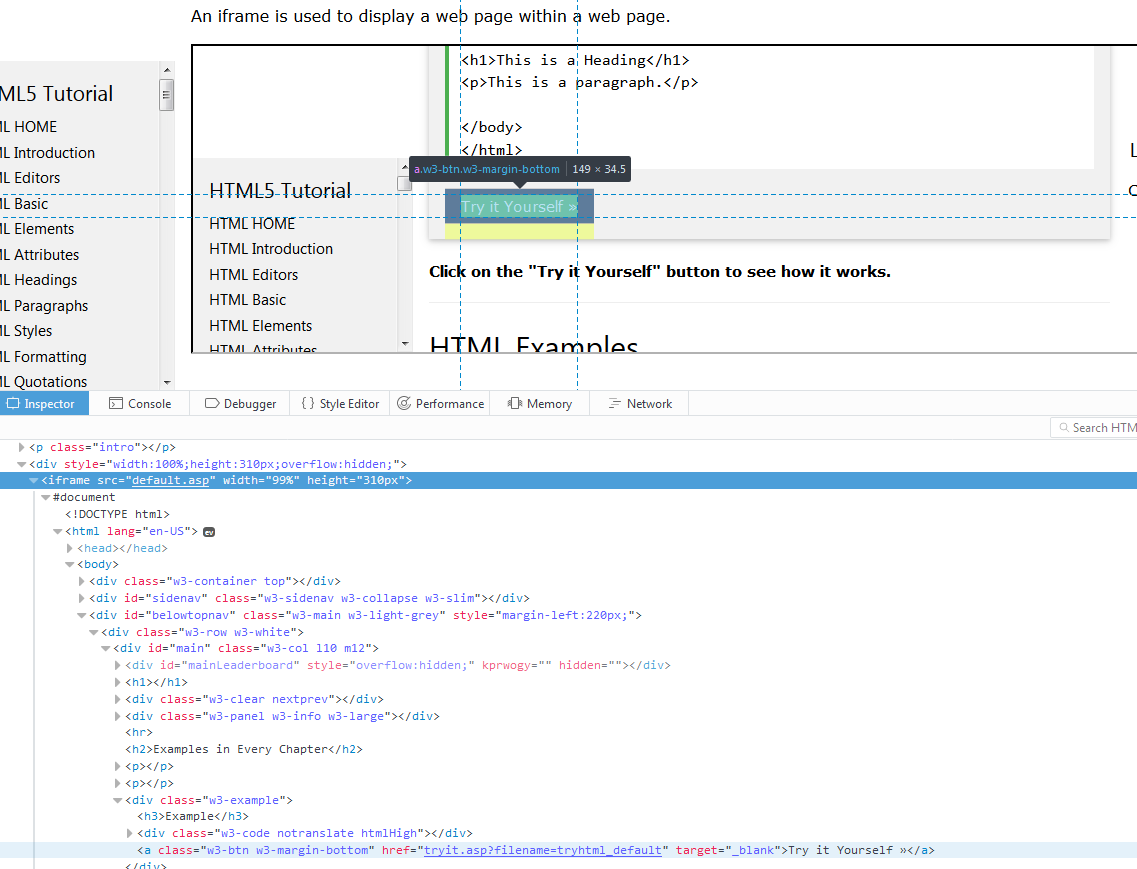
\includegraphics[scale=0.5]{instructions4}\newline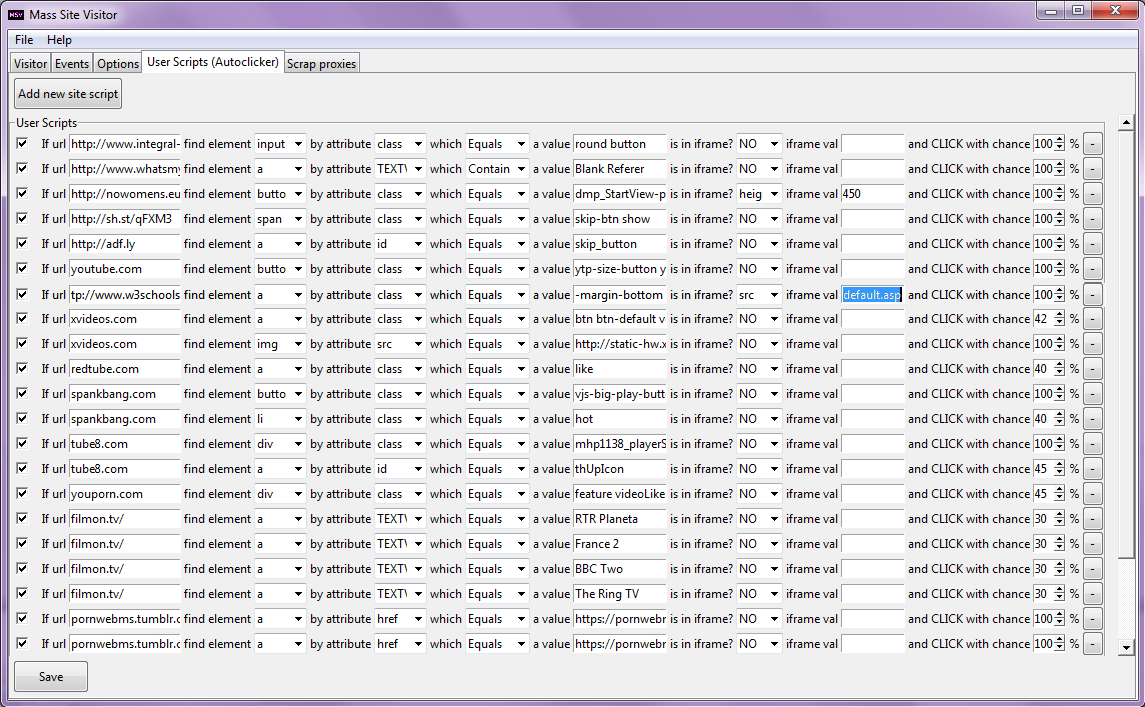
\includegraphics[scale=0.5]{instructions5}} 
\cvitem{\textbf{}}{As we can see in the example above we have ourselves a sticky situation: there's a neat little link we want to click, but it's from an embedded page within our target page, we can verify that by seeing that one of the parents in the html hierarchy of that link is an iframe element. That's why we have typed "\textit{\underline{src}}" as an "answer" to the "is in iframe?" question, and set the value of this \textit{\underline{src}} attribute as we observed in the browser's Element Inspector. If the keyword \textit{\underline{NO}} is used - target element is considered not a part of any iframe and is sought in the main page. In case something else is typed there (that drop-down menu is typable) - it will be considered an \underline{attribute} of an iframe to seek, and the next textfield will define the \underline{value} of that attribute.} 

%----------------------------------------------------------------------------------------
%	REFERRERS, TRAFFIC SOURCES SECTION
%----------------------------------------------------------------------------------------

\setlength{\hintscolumnwidth}{1.7cm}
\section{Google Analytics traffic sources}
\cvitem{}{The \textbf{JavaScript referrer injection} section of Options allows you to enable and somewhat customize spoofing of the referrer for Google Analytics. When this option is enabled, you'll see all the referrers, which you have loaded into the main tab (Visitor) of the program, appearing in the \textit{Traffic Sources} subsection of \textit{Real-Time View} in Google Analytics after starting the visitor. Default referrers, supplied with the bot include sources like google.com, fb.com, t.co, which are considered either an \textit{Organic} type of visitors (meaning from some search engine), or a \textit{Social Media} type by Google Analytics. Tweaking \textbf{injection timeout delay} might be helpful, because this feature slows down loading time, and might need to be kept in a relatively high value range (20+ seconds). Note: quite a few public proxies have a nasty habit of stripping referrers, so you have a chance of having about a quarter of your traffic as a (direct) source.} 

%----------------------------------------------------------------------------------------
%	TESTING PROXIES SECTION
%----------------------------------------------------------------------------------------

\section{Testing proxies}
\cvitem{}{You can test all the loaded proxies, using the \textbf{Test proxies} button in the \textit{Visitor tab}. It will use the \textbf{Proxy health} settings from the \textit{Options tab} like max proxy timeout, number of connection attempts (before discarding it as broken), and a minimal size of a correct response (in bytes), which is needed in case proxy reports that it's overloaded or doesn't allow you access via some typically small error page. Test is conducted by visiting url google.com from each of the proxies, until the list is exhausted, using the number of threads as set in the textfield of the \textit{Visitor tab}. If you allow proxies to have a high timeout, and have a big list of proxies, it might take a while to test all of them. But you typically would want to allow proxies to have rather high latency (slow response time), because you'll most likely run the bot for at least a couple of hours, gradually creating views. After the test is completed, you'll use \textbf{Settings - Export Healthy Proxies} to save good proxies into a text file. } 

\newpage

%----------------------------------------------------------------------------------------
%	MEDIA VIEWS SECTION
%----------------------------------------------------------------------------------------

\section{Influencing view count on media sharing sites (videos, audio streams)}
\cvitem{}{If you want to increase views of your video on some media sharing site, or of your channel on some audio streaming site, you quite possibly will need to visit those web-pages with a browser that supports video/audio playback (like Chrome), which is impossible in a headless browser, that is invisible and runs in a background. If you have \underline{Chrome browser installed on your PC}, you can choose to use it to visit the page on a media sharing site of your choice. The drawback of it is that there will be as many Chrome windows open, as there are of visitor running, \underline{however} they all are muted, and as you choose Chrome to be visitor's browser you will have a checkbox at the top of the \textit{Visitor tab} to hide all the Chrome windows off-screen. \textit{Pro-tip:} Disable JS referrer injection in the \textit{Options tab}, you probably won't need it for this purpose. Note: YouTube seems to discard anonymous views after certain amount, so you'll have tough luck seriously influencing YouTube views in particular.} 

%----------------------------------------------------------------------------------------
%	PROXIES SECTION
%----------------------------------------------------------------------------------------

\section{Private, socks proxies}
\cvitem{}{As it was mentioned above, a special keyword \underline{\textit{socks5}} is used in the same line as an ip of a socks4/5 proxy in the textfile, where you store all your proxies.} 
\cvitem{}{Private proxies require user authentication, and to fill in the username for the proxy server you will use the following construct in the same line of the text file as the proxy ip, separated from the address by a whitespace: \underline{\textit{u:whatvermyusername}}. The story is similar with the password: \underline{\textit{p:MySUp3R\$3CuR3pa\$\$W0rD}}. Take a look at these example lines:} 
\cvitem{}{127.0.0.1:80 socks5\newline
	127.0.0.1:80 u:myveryspecialname p:MySUp3R\$3CuR3pa\$\$W0rD\newline
	127.0.0.1:80 socks5 u:myveryspecialname p:MySUp3R\$3CuR3pa\$\$W0rD} 

%----------------------------------------------------------------------------------------
%	USER AGENTS SECTION
%----------------------------------------------------------------------------------------

\section{User agents, and client types (mobile, desktop) explained}
\cvitem{}{User agent string determines fully what kind of user is visiting the site: his operating system, device type and a browser client. Take a look at the examples below to clarify how the whole thing works.} 
\cvitem{}{A simple web search for some relevant up-to-date user agent string of typical users will yield you any desired results, just save them all into one text file, placing each such string into an independent line, and you are good to go, just don't forget to load it into the program.}
\cvitem{}{This string is \underline{Chrome} under \underline{Windows 7}: \textit{Mozilla/5.0 (Windows NT 6.1) AppleWebKit/537.36 (KHTML, like Gecko) Chrome/41.0.2228.0 Safari/537.36}\newline\newline
This one is \underline{Chrome} under \underline{OSX}: \textit{Mozilla/5.0 (Macintosh; Intel Mac OS X 10\_10\_1) AppleWebKit/537.36 (KHTML, like Gecko) Chrome/41.0.2227.1 Safari/537.36}\newline\newline
And here's a \underline{mobile} \underline{Chrome} user agent string: \textit{Mozilla/5.0 (Linux; Android 4.0.4; Galaxy Nexus Build/IMM76B) AppleWebKit/535.19 (KHTML, like Gecko) Chrome/18.0.1025.133 Mobile Safari/535.19\newline} 
}
\newpage
%----------------------------------------------------------------------------------------
%	COOKIE SECTION
%----------------------------------------------------------------------------------------

\section{Using cookies with MSV}
\cvitem{}{The cookies you want to use with MSV's visits need to be place in a json file, which has an array of cookie objects. See the json code listing below for example (this code is provided with the default cookie file, which is saved as cookies.json in the MSV user config folder, usually C:/Users/USERNAME/Mass Site Visitor). You can place all cookies for a multitude of domains, and only cookies for domains which are relevant to the current visited website will be applied to the visit. The ".domainname.com" with a leading dot is the most common way to set cookie domains, as the "." signifies that the cookie is applicable to all subdomains.} 
\cvitem{}{For most applications it might be enough to only set the "domain", "name" and "value" for a cookie. For more intricate cases - research the cookie fields, what they do, and which values they should have for your particular case.}
\begin{lstlisting}
[
		{
			"domain": ".mysite.com",
			"expirationDate": 1900835555.715111,
			"hostOnly": false,
			"httpOnly": true,
			"name": "Cookie1Name",
			"path": "/",
			"secure": true,
			"session": false,
			"storeId": null,
			"value": "COOKIE1VALUE"
		},
		{
			"domain": ".mysite.com",
			"expirationDate": 1901094435.295435,
			"hostOnly": false,
			"httpOnly": true,
			"name": "Cookie2Name",
			"path": "/",
			"secure": true,
			"session": false,
			"storeId": null,
			"value": "COOKIE2VALUE"
		}
]
\end{lstlisting}

\newpage

%----------------------------------------------------------------------------------------
%	QnA SECTION
%----------------------------------------------------------------------------------------

\setlength{\hintscolumnwidth}{4.4cm}
\section{FAQ: Common questions answered}
\cvitem{\textbf{1. Why can't I get any visits from the bot?}}{This may be happening for one of the few most common reasons:\newline
	1. Your firewall/anti-virus is blocking MSV from communicating with browsers it depends on.\newline
	2. Your IP/provider/region is blocked by some public proxies (due to your neighbor's involvements in spam, for instance), or you ISP might be blocking your access to some of the public proxies, and all of that is happening while \textbf{thread count} you've set is low, so try increasing it, to get to some responsive proxies faster and filter through unhealthy ones.\newline
	3. You didn't \textbf{scrap(re-scrap) new proxies}. See, if you are using public proxies, even if your list was working perfectly last week, doesn't mean it will today - public proxies tend to expire.\newline
	4. You didn't \textbf{update browser drivers}. There is a button for it in the Visitor tab, or you can download them manually and place into the bin/ folder of the MSV distro.\newline
	5. Your website is captcha-protected, and the protection provider reacts aggressively to public proxies. MSV doesn't solve captcha. So in this case, disable the protection temporarily to send bot views, or use private paid proxies, which won't trigger the protection.} 

\cvitem{\textbf{2. How do I reduce bounce rate?}}{Bounce rate is battled best by clicking on a link, which leads to some \textbf{other} page of the \textbf{same} website you're targeting. Clicker feature (Auto-Random Behavior and/or specific User Scripts), described above in this manual, suits this task perfectly.} 

\cvitem{\textbf{3. How much traffic is it possible to generate?}}{Speed depends highly on the proxies (how many of them are responsive and how much do they lag), and bottle-necked by your ram (how many browsers will you be able to run in a background simultaneously). With public proxies and 8 GB of RAM I was able to run 50 threads, and get like 400 views an hr. Though it can be \textbf{much} higher, if proxies are responsive and fast; or can be even worse, if no good proxies are at hand. In daily terms it will fluctuate from couple of 1000's, to couple of 10000's on average for an average desktop PC. But sky is the limit here, if you have access to a lot of fast responsive proxies and a top-tier hardware} 

\cvitem{\textbf{4. How can I influence keywords in GA?}}{You could try setting referrers for Google keywords, you might need to use a weird link like this: https://www.google.com/url?sa=t\&rct=j\&q=\&esrc=s\&source=web\&cd=1\&cad=rja\newline
	\&uact=8\&ved=2ahASDwqwer\_ASdasdQWEEQWEASDasdQWE\newline
	\&url=https\%3A\%2F\%2Fwww.asp.net\%2Fmvc\newline
	\&usg=ASDwqeASdwqeqdafASD\_3asdASDASdasd , which is the link, that leads to your site from Google search page, if you are ranking at google.\newline
Though sometimes simpler referrers might work like https://www.google.com/?q=keyword1+keyword2. But it's not always working.\newline
Alternatively, visit Google search page, where your site is ranking, set the bot to click on the search result, that way correct keywords will most likely register in GA.}  

\cvitem{\textbf{5. I want to click on google ads. How to setup User Scripts? With ads, classes are constantly changing, which attribute/tag do I use?}}{Depends on the ad provider used, really. You can also use “Contains” selector (instead of “Equals”) with MSV for the value of attribute, if for instance “class” attribute always has a different value, but some part of it is always present. You can also use any other attribute, not necessarily “class”. Also, if you are placing your ads into a “div” container, you can give it and “id” and try setting a click on that “div” by its “id”. Just make sure that the div isn't larger than the ad, and doesn't contain anything besides the ad. Usage of other container tags, other than “div” is also possible.}  

\cvitem[0.5em]{\textbf{6. Events tab error: ‘Error launching a’, ‘Chrome’, ‘browser.’, WebDriverException(‘unknown error: failed to wait for extension background page to load: chrome-extension://cknebhggccemgcnbidipinkifmmegdel/html/background.html from unknown error: page could not be found: chrome-extension://cknebhggccemgcnbidipinkifmmegdel/html/background.html’, None, None)}}{Try disabling the Alexa addon, or disabling headless mode for Chrome (if you need to have the Alexa addon enabled).}  

\cvitem{\textbf{7. I try to use a long url referral but it’s not working}}{The standard referrer list, provided with MSV contains http://t.co as referrer, if you are only interested in twitter as referrer, use the list that contains just that link, because as far as i know, twitter processes all it’s external links through t.co domain, an all twitter referrers pretty much look like that. Don’t forget to enable the JS referrer injection option, like it is shown at the beginning of the demo 3 video, it’s needed for different JS-based analytics (like GA). Also, some public proxies like to strip the referrer, so some of your traffic will end up being direct no matter what (but the percentage will be at most 20\%, like in the demo videos).}  

\cvitem{\textbf{8. From your experience, what are the best selections (in options panel) in order to get more pageviews in GA ?}}{I’d say if traffic sources matter to you – have JS injection option enabled, it’ll slow down page loading, but referrers will get registered in GA. Have proxy timeout to somewhat above a minute if you’re using public proxies – a lot of the lag, but tend to respond after waiting for a while.For bounce rate – set the bot to click on some link, which leads to a different page on the target website, therefore making it look like the visitor didn’t just bounce (entered some page and left without checking the rest of the website). Have page stay intervals for like 5-15 secs or something like that, it will be slightly slower, but if you have some extra javascript on the page – the delay might help to load page more fully before leaving/doing a click. Unless Alexa rank and/or video/audio playback matters – just use headless Chrome. If you don’t have any problems – just disable page snapshot saving – they are only useful for diagnosing how the target page was loading (especially yin the headless browser).}  

\cvitem{\textbf{9. Will it increase website rank in Google or Alexa rank?}}{Google ranking is more complex than that, backlinks are a factor, and for long term high ranking you need quality content on your site and returning users. BUT traffic bots and tweaking your GA stats sure will have a boost for your ranking. Alexa rank can be influenced with Alexabar add-on, and non-headless chrome, or Firefox.}  

\cvitem{\textbf{10. Are 32-bit systems supported?}}{MSV is a 64 bit only software, and due to high RAM requirements, using less than 8 GiB (32 bit being constrained to 4 GiB) isn't going to get you very far.}  

\cvitem{\textbf{11. Any Google Analytics-specific settings for MSV?}}{Any browser + JS injection option enabled is perfect for GA.}  

\cvitem{\textbf{12. Can I increase my Alexa rank using MSV?}}{Yeah, using Alexa addon option Firefox + Js injection + Alexa add-on used to be the go-to combo for Alexa, but non-headless chrome might be better.}    

\cvitem{\textbf{13. Google ad clicking questions}}{If you are thinking about clicking ads on your sites with bot traffic I would like to at least discourage you from doing so from public proxies. Any PPA network is a bit too smart for such obvious tricks, and the amount of money gained from using bot clicks will not out-weight the significant chance of being banned and never seeing your \$10, which the bot traffic created you over a couple of days I guess if you have some private proxies (but those cost money, and you have to seek out providers with ‘unsullied’ IPs, which nobody else used for some kind of spam or whatever) that might yield some modest results.}    

\cvitem{\textbf{14. Can i use MSV for bitly short links?}}{Kind of yeah, clicker feature will be helpful for you, but the risk to get banned is pretty significant But it’s risky, and you have to start small, and there will always be a chance to get banned. Clicker feature of MSV lets you press those skip ad/continue links like a real user would.}  

\cvitem{\textbf{15. Does your bot clicks on Google Ads?}}{You can set the bot to click on as links and banners, etc. But it could get you banned. Your clicks to ads essentially never convert – obviously fake bot click cannot make a real purchase with real money, the ad provider might see at a very suspicious trend.}

\cvitem{\textbf{16. Is it safe for AdSense websites?}}{Yes, it doesn't click on ads by default.}

\cvitem{\textbf{17. I want to use MSV to click my competitor ads on Amazon by searching the product on there and clicking ads.}}{ If their products are available on the search page, then it should be doable by:1 targeting in msv url amazon.com/some-kind-of-search-url2 using instructions in the PDF manual, setting the bot to click on ad on the search page, it will work if your competitor’s ads have like a unique id, or text or something in the HTML code of the page. You can check that out using browser inspection.}

\cvitem{\textbf{18. Can MSV do several websites at a time?}}{ You can enter several websites, one per line in the Visitor tab, to be visited simultaneously.}

\cvitem{\textbf{19. Country-specific traffic, targeting particular countries}}{ You can scrap proxies from any country of your choice from several free proxy websites using MSV, which will make the generated traffic country-specific. You can also load your own list of any proxies from any countries. Locales are available also, you can set browser language, works best for Chrome or Firefox.}

\cvitem{\textbf{20. Does your tool have the Anti-fingerprint? To bypass bot detection?}}{ Sessions are always distinct, so fingerprinting is not likely. Additionally, obfuscation techniques are applied to prevent bot detection.}

\cvitem{\textbf{21. Driver version error in the Events tab of MSV.}}{ Well the error says that you have mismatch between chrome and chrome driver, so either press the update browser drivers button on the main window, or see the about window for links to chrome driver and download the one according to your chrome version, and replace it in bin folder of MSV. You should download the latest versions of those drivers from the official web-sites, check these links https://github.com/mozilla/geckodriver/releases https://sites.google.com/a/chromium.org/chromedriver/downloads.}

\cvitem{\textbf{22. How to use it?}}{ Just unpack the archive into some folder, run the .exe file, scrap proxies, enter website url, press start, consult the PDF manual for any specific questions, or by checking out and studying the gui (it also has hints) – it should be pretty self-explanatory.}

\cvitem{\textbf{23. Can i use Mass Site Visitor for YouTube url?}}{ YouTube is not properly supported – i don’t guarantee any impressive results there, however I was able to pump a few hundreds of views on some fresh videos. Non-headless browser, auto-random clicking and scrolling should be helpful here as well.}

\newpage

%----------------------------------------------------------------------------------------
%	REQUIREMENTS SECTION
%----------------------------------------------------------------------------------------

\setlength{\hintscolumnwidth}{1.7cm}
\section{Requirements, gotchas}

\cvitem{1}{Program should run independently of any third party libraries and runtimes, tested on a clean install of Windows 8.1 and 10, you do need to have browsers like Chrome and Firefox installed, however.} 

\cvitem{2}{The program itself communicates with the headless browser through the socket interface, so to allow inter-process communication you will most likely have \textbf{to allow Windows Firewall to give both PhantomJS and MSV the green light} (usually, firewall will straight up ask if you want to allow the program to communicate through network).}

\cvitem{3}{You might get it working on \textbf{Windows XP}, but MSV was never tested on it.}

\cvitem{4}{The folder will all the settings and outputs will be something like C:/Users/Your Username/Site Mass Visitor. If you never changed the default directory of saving scraped proxies, they are in that folder somewhere.}

\cvitem{5}{The software was tested on a computer with i5 Processor and 8 GiB or RAM. With that said, for all the video previews, which where recorded while the bot was running 35 threads, with browser playing youtube videos in the background and me playing a videogame on the second monitor at the time, everything was very smooth. And I use about 40+ threads most of the time for my purposes. For \textit{\underline{low-end}} machines \textbf{thread count} customization exists in the program right in the main tab for a reason. Adjust it according to the performance possible with your machine. Disable \textbf{snapshot saving} as well, to save your PC the trouble of numerous disk writing operations. Remember, that 50 instances of even a headless browser will take about 6 GiB of RAM.}

\cvitem{6}{Blank lines. Sometimes you want some of your visits to come with a blank referer field, or even with your direct ip without a proxy. For this case just put an "extra" newline (in between some filled lines with user agents/proxy IPs, or press "Enter" twice when on the last filled with data line), such line will be interpreted as an empty string, and will either be used as a referer, or just connect to the web-site directly without proxy, in case that the line will be selected randomly.}

\cvitem{7}{Browser window dimensions. In the \textit{Options menu} you can see a textfield, which will by default have a few lines present, each representing \textit{width x height} pair for a window dimensions, chosen randomly at runtime for web-site visits, use exactly this format of one per line WIDTHxHEIGHT number pairs.}

\cvitem{8}{\textbf{Alexa toolbar/extension}. Alexa extension has shown instabilities with Chrome: when several threads (often even just one) are running, Alexa bar can fail to be installed properly (doesn't happen all the time - doesn't appear to have any system to it), and what's worse is that session creation fails because of it, and what's even worse is that it doesn't close the browser window automatically. Possible solutions are being tested yet, but are imperfect: i.e. having a profile with pre-installed Alexa extension to be reused creates fingerprint. So possibly I would have to wait for new chromedriver/chrome release for that to get fixed. In the meantime you should stick to Firefox (Nightly as explained in the following section).}

\cvitem{9}{\textbf{Firefox (geckodriver)}. It is highly recommended to have Nightly version installed/available on your system, instead of the regular Firefox. When the regular or even developer editions were tested, crashes were happening regularly during attempts to simply close the browser. Nightly doesn't suffer from such problems at all and was proven to be stable Windows 7, 8.1 and 10.}


\end{document}